% fig:teaser V3 -- single-column page-1 teaser
% Self-contained TikZ. Design width 8.2 cm = \columnwidth; fonts at native
% size (no \resizebox). Schematic icons only, no real faces.
% Toggle in main.tex: \TeaserEnabledtrue / \TeaserEnabledfalse.
\centering
\definecolor{tzBlue}{RGB}{47,76,166}
\definecolor{tzOrange}{RGB}{214,116,34}
\definecolor{tzGray}{RGB}{95,100,110}
\definecolor{tzDark}{RGB}{45,50,60}
\definecolor{tzRed}{RGB}{186,62,54}
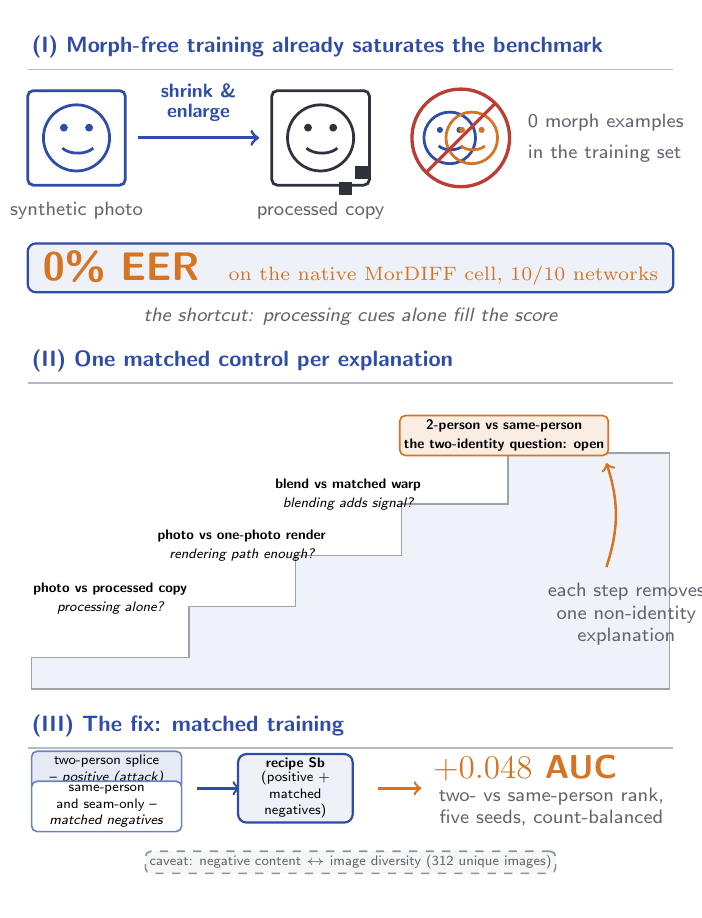
\begin{tikzpicture}[
  x=1cm,y=1cm,
  font=\sffamily,
  every node/.style={align=center, inner sep=1.5pt, outer sep=0pt},
  fline/.style={line width=1.0pt},
  hrule/.style={draw=tzGray!45, line width=0.6pt},
  boxR/.style={draw=tzBlue, fill=tzBlue!8, rounded corners=3pt, line width=0.8pt},
  chip/.style={draw=tzBlue!70, rounded corners=2pt, line width=0.6pt, fill=white},
  caveat/.style={draw=tzGray!70, dashed, rounded corners=2pt, line width=0.6pt,
                 fill=tzGray!6, text=tzGray},
  head/.style={anchor=west, font=\sffamily\bfseries\footnotesize, text=tzBlue},
  hint/.style={font=\sffamily\scriptsize, text=tzGray},
  qlab/.style={font=\sffamily\scriptsize\itshape, text=tzGray},
]
\useasboundingbox (0,0) rectangle (8.2,10.95);

% ------------------------------------------------------------- icons
\tikzset{
  picface/.pic={
    \draw[fline, pic actions] (0,0) circle (0.42);
    \fill[pic actions] (-0.16,0.13) circle (0.05);
    \fill[pic actions] (0.16,0.13) circle (0.05);
    \draw[fline, pic actions] (-0.18,-0.13) arc (215:325:0.24 and 0.15);
  },
}

% ============================================================== ACT I
\node[head] at (0.0,10.70) {(I) Morph-free training already saturates the benchmark};
\draw[hrule] (0.0,10.42) -- (8.2,10.42);

% pipeline row
\begin{scope}[shift={(0.62,9.55)}] \path pic[tzBlue] {picface}; \end{scope}
\draw[fline, tzBlue, rounded corners=2pt] (0.0,8.95) rectangle (1.24,10.15);
\node[hint] at (0.62,8.62) {synthetic photo};
\begin{scope}[shift={(3.72,9.55)}] \path pic[tzDark] {picface}; \end{scope}
\draw[fline, tzDark, rounded corners=2pt] (3.10,8.95) rectangle (4.34,10.15);
\fill[tzDark] (3.96,8.83) rectangle (4.12,8.99);
\fill[tzDark] (4.16,9.03) rectangle (4.32,9.19);
\node[hint] at (3.72,8.62) {processed copy};
\draw[->, tzBlue, line width=1.1pt] (1.40,9.55) -- (2.94,9.55);
\node[font=\sffamily\scriptsize\bfseries, text=tzBlue] at (2.17,10.00)
  {shrink \&\\[-1pt] enlarge};
\begin{scope}[shift={(5.50,9.55)}]
  \path (-0.14,0) pic[scale=0.78, tzBlue] {picface};
  \path (0.14,0)  pic[scale=0.78, tzOrange] {picface};
  \draw[tzRed, line width=1.2pt] (0,0) circle (0.62);
  \draw[tzRed, line width=1.2pt] (-0.44,-0.44) -- (0.44,0.44);
\end{scope}
\node[hint, anchor=west] at (6.30,9.75) {0 morph examples};
\node[hint, anchor=west] at (6.30,9.35) {in the training set};
% hero number
\node[boxR, font=\sffamily\bfseries\fontsize{14}{15}\selectfont, text=tzOrange,
      minimum height=0.62cm, minimum width=8.2cm] at (4.10,7.90)
  {0\% EER\ \ {\normalfont\scriptsize on the native MorDIFF cell, 10/10 networks}};
\node[qlab] at (4.10,7.28) {the shortcut: processing cues alone fill the score};

% ============================================================== ACT II
\node[head] at (0.0,6.72) {(II) One matched control per explanation};
\draw[hrule] (0.0,6.44) -- (8.2,6.44);

% staircase: four steps
\fill[tzBlue!7] (0.05,2.55) -- (0.05,2.95) -- (2.05,2.95) -- (2.05,3.60)
  -- (3.40,3.60) -- (3.40,4.25) -- (4.75,4.25) -- (4.75,4.90)
  -- (6.10,4.90) -- (6.10,5.55) -- (8.15,5.55) -- (8.15,2.55) -- cycle;
\draw[tzGray!60, line width=0.5pt] (0.05,2.55) -- (0.05,2.95) -- (2.05,2.95)
  -- (2.05,3.60) -- (3.40,3.60) -- (3.40,4.25) -- (4.75,4.25) -- (4.75,4.90)
  -- (6.10,4.90) -- (6.10,5.55) -- (8.15,5.55) -- (8.15,2.55) -- cycle;
% tread chips (inside each step, no overlap)
\node[font=\sffamily\tiny] at (1.05,3.70) {\textbf{photo vs processed copy}\\[1pt]
  {\itshape processing alone?}};
\node[font=\sffamily\tiny] at (2.72,4.37) {\textbf{photo vs one-photo render}\\[1pt]
  {\itshape rendering path enough?}};
\node[font=\sffamily\tiny] at (4.07,5.02) {\textbf{blend vs matched warp}\\[1pt]
  {\itshape blending adds signal?}};
\node[font=\sffamily\tiny, draw=tzOrange, fill=tzOrange!12, rounded corners=2pt,
      line width=0.6pt] at (6.05,5.77) {\textbf{2-person vs same-person}\\[1pt]
  {\bfseries\itshape the two-identity question: open}};
% note pointing to ladder
\node[hint, anchor=west, text width=2.0cm] at (6.55,3.50)
  {each step removes one non-identity explanation};
\draw[->, tzOrange, line width=0.9pt] (7.35,4.10) to[bend right=18] (7.35,5.42);

% ============================================================== ACT III
\node[head] at (0.0,2.08) {(III) The fix: matched training};
\draw[hrule] (0.0,1.80) -- (8.2,1.80);

% left: the three training ingredients
\node[chip, fill=tzBlue!12, anchor=west, font=\sffamily\tiny,
      text width=1.80cm] at (0.05,1.52)
  {two-person splice -- \emph{positive (attack)}};
\node[chip, anchor=west, font=\sffamily\tiny, text width=1.80cm] at (0.05,1.06)
  {same-person and seam-only -- \emph{matched negatives}};
\draw[->, tzBlue, line width=0.9pt] (2.15,1.29) -- (2.70,1.29);
% center: recipe
\node[boxR, font=\sffamily\tiny, text width=1.35cm] at (3.40,1.29)
  {\textbf{recipe \textsf{Sb}}\\[-1pt](positive +\\ matched negatives)};
\draw[->, tzOrange, line width=0.9pt] (4.45,1.29) -- (5.00,1.29);
% right: headline number
\node[font=\sffamily\bfseries\fontsize{13}{14}\selectfont, text=tzOrange,
      anchor=west] at (5.10,1.55) {$+0.048$ AUC};
\node[hint, anchor=west, text width=3.0cm] at (5.10,1.05)
  {two- vs same-person rank, five seeds, count-balanced};
% caveat, own row, centered
\node[caveat, font=\sffamily\tiny] at (4.10,0.35)
  {caveat: negative content $\leftrightarrow$ image diversity (312 unique images)};

\end{tikzpicture}
